\documentclass[a4paper,11pt]{jsarticle}


% 数式
\usepackage{amsmath,amsfonts}
\usepackage{bm}
% 画像
\usepackage[dvipdfmx]{graphicx}
\usepackage[dvipdfmx,setpagesize=false,hidelinks]{hyperref}
% \usepackage{svg}

\usepackage{autobreak}
%図の位置の操作
\usepackage{float}

\setlength{\voffset}{-20mm}
\setlength{\textheight}{230mm}

\renewcommand{\figurename}{Fig.}
\renewcommand{\tablename}{Table}


% \usepackage{pxjahyper}


\begin{document}

\title{制御工学特論 中間レポート}
\author{青木敦郎}
\date{\today}
\maketitle

\section{はじめに}
Roombaは差動2輪駆動のロボットであり,左右のタイヤを駆動させるモーターに任意のPWM信号を送ることで,タイヤが回転しRoombaを移動させることができる.
Roombaに標準で搭載されているロータリーエンコーダからタイヤの回転数を取得し,オドメトリの計算によりRoombaの位置と姿勢を推定することができる.
Roombaを様々な軌道で移動させる際,オドメトリによる位置姿勢等の値と,実際の値の差異を比較することが本レポートの目的である.\par
実際の位置姿勢等を取得する方法としては,モーションキャプチャーにより位置姿勢を取得する方法を採用する.

\section{直進性能評価実験}

\subsection{目的}
この実験では,Roombaを任意の時間だけ直進運動させたとき,オドメトリにより算出された結果と,実際の座標等から得られた結果を比較し考察する.
考察内容としては,オドメトリにより推定されるRoombaの軌跡と実際の軌跡との比較を行う.
また,進んだ距離に対して姿勢の変化をオドメトリの姿勢と実際の姿勢で比較を行う.

\subsection{実験方法}
Roombaにモーションキャプチャー用のマーカーを載せる.
Roombaの左右のモーターに同じ大きさのPWM信号を一定時間送り続ける.
取得したロータリーエンコーダの値から,オドメトリによりRoombaの位置姿勢を推定し,記録する.
また,モーションキャプチャーから得られた位置姿勢についても記録する.\par
オドメトリから推定された値とモーションキャプチャーで得られた値について,
それぞれの位置と距離に対する姿勢を比較する.

\subsection{結果}
オドメトリから推定された値とモーションキャプチャーで得られた値から,結果をFig.{\ref{fig:1}},Fig.{\ref{fig:2}}に示す.
各グラフにおける凡例の"Capture"は,モーションキャプチャーにより得られた値を参照しており,"Odometry"はオドメトリにより得られた値を参照している.\par
Fig.{\ref{fig:1}}では,オドメトリにより得られた座標にモーションキャプチャーで最初に得られたRoombaの姿勢角度の補正を入れ,
モーションキャプチャーにより得られた座標には最初に得られた位置を原点とするような補正を入れている.
また,Fig.{\ref{fig:2}}のモーションキャプチャーで得られた値は,小数点以下を四捨五入している.\par
Fig.{\ref{fig:1}}からは,オドメトリにより得られた軌跡とモーションキャプチャーにより得られた軌跡でずれが見受けられる.
このずれは,Fig.{\ref{fig:1}}の原点からX軸の正の方向に進むと大きくなっていることが分かる.
Fig.{\ref{fig:2}}より,移動し始めた地点でのオドメトリによる姿勢は,モーションキャプチャーによる姿勢と比べ遅れて一致していることが分かる.

\begin{figure}[H] %\begin{figure}[画像の配置場所]
        \begin{center}
        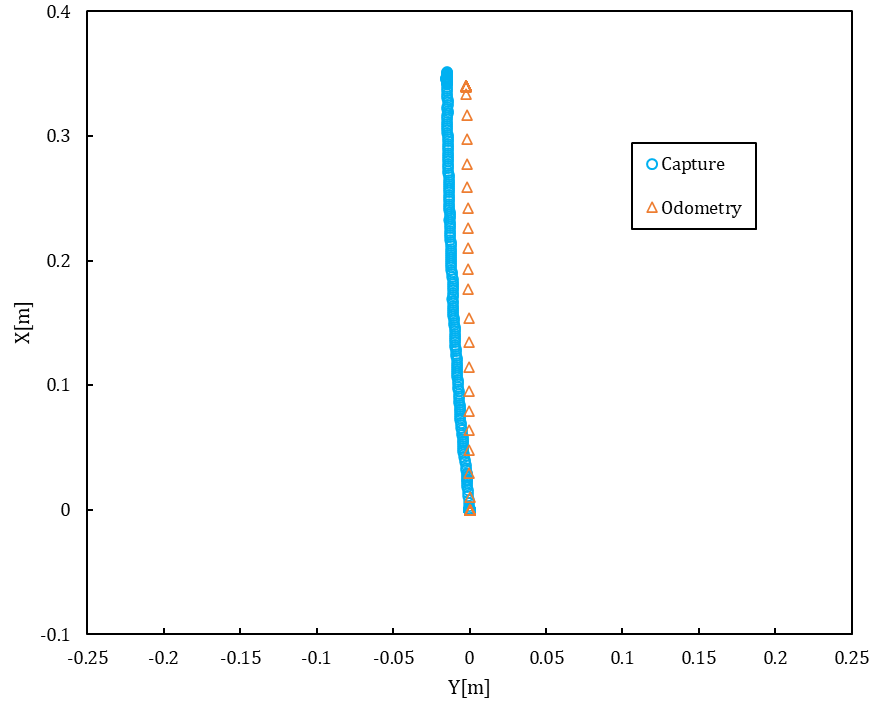
\includegraphics[width=100mm]{../graph/Xvs.Y.png}
        \caption{Roombaの軌跡}%図の説明
        \label{fig:1}
        \end{center}
\end{figure}
\begin{figure}[H] %\begin{figure}[画像の配置場所]
        \begin{center}
        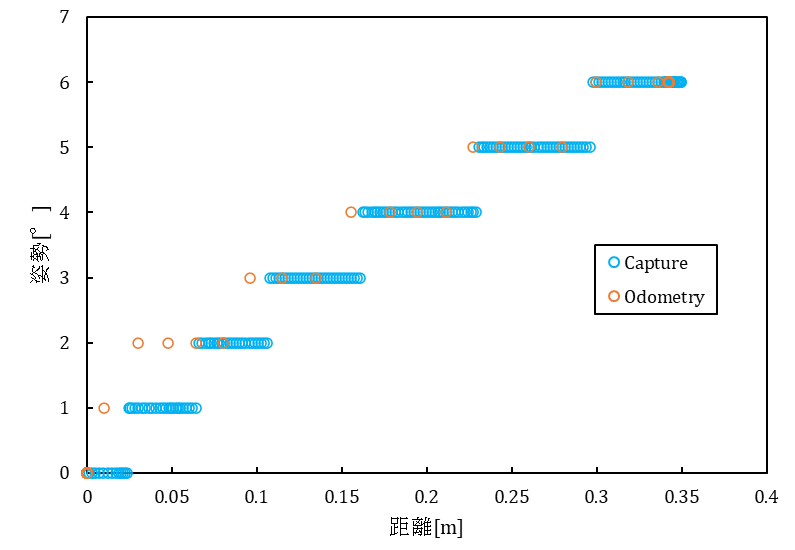
\includegraphics[width=100mm]{../graph/Rotationvs.Distance.png}
        \caption{距離と姿勢の関係}%図の説明
        \label{fig:2}
        \end{center}
\end{figure}

\subsection{考察}
Fig.{\ref{fig:1}}において見受けられたずれは,Roombaのタイヤの滑りとオドメトリの計算によって生じたものである.
Fig.{\ref{fig:2}}では,距離が大きくなるにつれ,姿勢が一致しやすくなっている.静止状態から走り始めは静止摩擦が大きく,その分大きなトルクが必要となる.
大きなトルクにより走り始めるため,左右のタイヤの滑り具合が異なり,姿勢もその分ずれが生じるためである.\par
また,Fig.{\ref{fig:2}}の移動し始めた地点での,オドメトリとモーションキャプチャーで取得したそれぞれの姿勢のずれは,
Fig.{\ref{fig:1}}での軌跡のずれとしても影響が表れている.
オドメトリで取得する座標は,過去に取得したタイヤの回転数を基に現在位置を更新するため,
Fig.{\ref{fig:2}}においての移動開始地点での姿勢のずれが残ったままオドメトリの計算が行われ,
結果としてFig.{\ref{fig:1}}では移動するにつれ座標のずれが大きくなった.


\section{\label{experi}その場旋回評価実験}

\subsection{目的}
この実験では,Roombaを任意の時間だけその場旋回運動させたとき,
オドメトリにより算出された姿勢と,
モーションキャプチャーから得られた姿勢を比較し考察する.
考察内容としては,オドメトリにより推定されるRoombaの姿勢と実際の姿勢の,
時間による変化の比較を行う.

\subsection{実験方法}
前述の実験と同様に,Roombaにモーションキャプチャー用のマーカーを載せる.
Roombaの左右のモーターに,同じ大きさでタイヤの回転方向が異なるようにPWM信号を送り続ける.
Roombaに信号を送ることで回転させ,これを元の姿勢と同じ姿勢になるまで回転させる.
取得したロータリーエンコーダの値から,オドメトリによりRoombaの姿勢を推定し,記録する.
また,モーションキャプチャーから得られた姿勢についても記録する.\par
オドメトリから推定された値とモーションキャプチャーで得られた値について,
それぞれの時間に対する姿勢を比較する.

\subsection{結果}
オドメトリから推定された値とモーションキャプチャーで得られた値から,結果をFig.{\ref{fig:RotTimturn}}に示す.
尚,このグラフは,オドメトリとモーションキャプチャーで測定を開始したタイミングにずれがあるため,開始のタイミングを調整している.
Fig.{\ref{fig:RotTimturn}}では,オドメトリとモーションキャプチャーの測定結果でオフセットがかかったようなずれが生じていることが分かる.
また,どちらの測定結果も回転し始める時の角度の変化は緩やかになっている.

\begin{figure}[H] %\begin{figure}[画像の配置場所]
        \begin{center}
        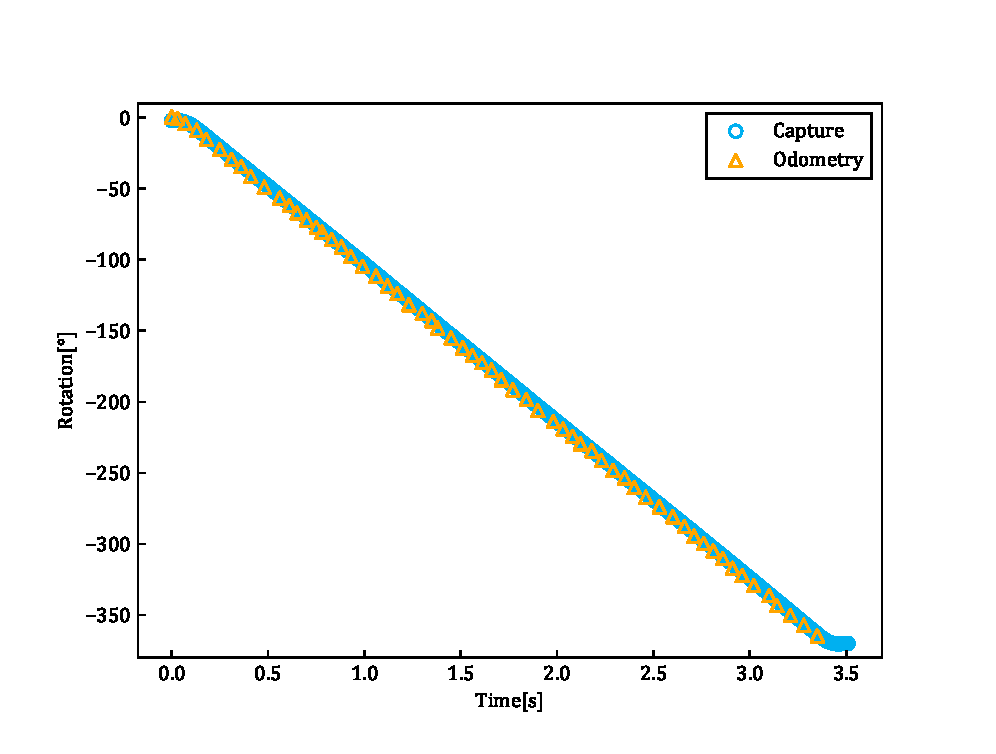
\includegraphics[width=100mm]{../graph/RotTimturn.eps}
        \caption{時間と姿勢の関係}%図の説明
        \label{fig:RotTimturn}
        \end{center}
\end{figure}

\subsection{考察}
Fig.{\ref{fig:RotTimturn}}より,オフセットがかかる原因は参照するタイミングがまだずれているためである.
また,回転開始の時間で角度の変化が緩やかになっているのは,Roombaが静止している状態から回転を開始し,
いきなり定常的な回転速度を得られずに徐々に回転速度を上げているためである.

移動しながらの旋回の評価,しっかりと旋回(姿勢が変化)できているか,オドメトリと実際はどうか,
\newpage
\section{おわりに}
Roombaを様々な軌道で移動させる際,オドメトリによる位置姿勢等の値と実際の値を比較する実験を,直進性能評価実験とその場旋回評価実験として行った.
実験を通して次のことが分かった.
\begin{itemize}
        \item Fig.{\ref{fig:1}}において見受けられたずれは,Roombaのタイヤの滑りとオドメトリの計算方法によって生じたものである.
        \item Fig.\ref{fig:2}からは静止状態から走行するため,左右のタイヤの摩擦の差により姿勢のずれが最初で大きくなっている.
        \item \hyperref[experi]{その場旋回評価実験}から,緩やかに旋回速度を上げて定常的な回転速度を得ている.
\end{itemize}
オドメトリは過去の値を用いて計算するため,移動する距離が大きくなるとともにずれも大きくなることが分かった.
また,タイヤの滑りもずれが大きくなる要因となる.これらのずれを考慮し,Roombaの位置姿勢を計算する必要がある.

\end{document}